\documentclass[11pt,a4paper]{article}

\usepackage[T1]{fontenc}
\usepackage[utf8]{inputenc}
\usepackage{lmodern}
\usepackage[a4paper,margin=2.3cm]{geometry}
\usepackage{amsmath}
\usepackage{graphicx}
\usepackage{booktabs,tabularx,array}
\usepackage{enumitem}
\usepackage{float}
\usepackage{caption}
\usepackage[hidelinks]{hyperref}

\setlist{itemsep=2pt,topsep=3pt}
\captionsetup{font=small,labelfont=bf}
\renewcommand{\arraystretch}{1.15}
\newcommand{\code}[1]{\texttt{#1}}
\setlength{\emergencystretch}{3em}

\title{\textbf{Project Log}\\[4pt]
\large RL-ROS2-waffle: PPO navigation training\\
\normalsize Branches \code{first\_PPO\_training} (Part I) and
\code{PPO\_evoution\_and\_tweaks} (Part II)}
\author{Jakub Wilczyński \and Maksymilian Tulewicz}
\date{4--12 November 2026}

\begin{document}
\maketitle

\part*{Part I: first PPO training (\code{first\_PPO\_training})}
\addcontentsline{toc}{part}{Part I}

% ======================================================================
\section{Summary}
% ======================================================================
The branch \code{first\_PPO\_training} (commits \code{6638d6f}, 3 Nov, and
\code{6b1a565}, 4 Nov, on top of \code{main} at \code{fcd4d5f}) turns the
existing simulation parts (scene generator, map generator, LiDAR, controller)
into a complete reinforcement-learning pipeline. The TurtleBot3 Waffle Pi now
learns with PPO (Stable-Baselines3) to drive to a goal on randomly generated
grid maps in MuJoCo. On the hardest evaluation maps the robot reaches the goal
in 20\% of episodes at the end of training (best: 40\%); most failures are
collisions.

% ======================================================================
\section{Changes}
% ======================================================================

\paragraph{Structure and packaging.} Modules moved from \code{src/} to the
installable package \code{src/tb3\_nav/}; \code{pyproject.toml} replaces
\code{requirements.txt} and adds Stable-Baselines3, TensorBoard and
Matplotlib. \code{pip install -e .} provides the commands \code{tb3-train},
\code{tb3-play}, \code{tb3-plot}, \code{tb3-show}, \code{tb3-layouts} and
\code{tb3-make-scene}.

\paragraph{Robot model and LiDAR.} The wheel velocity actuator gain was raised
from \code{kv=0.1} to \code{kv=1.0}, so the wheels follow the commanded speed.
A LiDAR ray that hits nothing now returns the maximum range (1.5\,m) instead
of $-1$, so normalised readings lie in $[0,1]$.

\paragraph{Gymnasium environment (\code{nav\_env.py}).} At every reset a new
map is generated on the $10\times10$ grid (0.5\,m cells) and the robot starts
at a random cell and heading. The action is applied for 25 physics steps
(0.05\,s, 20\,Hz control). The distance and angle to the goal in the robot
frame come from the new \code{geometry.py}.

\begin{table}[H]
\centering\small
\begin{tabularx}{\textwidth}{@{}l X@{}}
\toprule
Action (2) & $[v,\ \omega]\in[-1,1]^2$, scaled to 0.26\,m/s and 1.82\,rad/s \\
Observation (41) & 36 LiDAR readings, robot $v$ and $\omega$, distance to goal, $\sin$/$\cos$ of the angle to goal (all normalised) \\
Reward & $10\cdot$progress to the goal [m] $-\,0.01$ per step; $+15$ goal; $-15$ collision \\
Episode end & goal $\le 0.2$\,m; collision: LiDAR $\le 0.2$\,m; limit 500 steps (1500 in the last stage) \\
\bottomrule
\end{tabularx}
\caption{Definition of \code{NavEnv}.}
\end{table}

\paragraph{PPO training with curriculum (\code{train\_ppo.py}).} PPO with
4 parallel environments, $\gamma = 0.995$ (the goal is often 200--400 steps
away) and $256\times256$ policy and value networks. Training moves to the
next stage when the robot reaches the goal in 70\% of the last 100 episodes.
Evaluation always runs on the hardest stage. Every run is saved in its own
folder \code{runs/<date\_time>/} with the config, best and final model,
TensorBoard logs and plots.

\begin{table}[H]
\centering\small
\begin{tabular}{@{}c l c c c@{}}
\toprule
Stage & Map types & Obstacles & Min.\ start--goal distance & Step limit \\
\midrule
0 & random & 0--3 & 2 cells & 500 \\
1 & random & 3--8 & 3 cells & 500 \\
2 & random & 8--15 & 5 cells & 500 \\
3 & random, rooms, maze & 8--15 & 5 cells & 1500 \\
\bottomrule
\end{tabular}
\caption{Curriculum stages.}
\end{table}

\paragraph{Tools, tests, documentation.} \code{plot\_run.py} draws the training
curves from the TensorBoard logs; \code{play\_model.py} shows a trained model
driving in the MuJoCo viewer and counts goals, collisions and timeouts. New
tests cover the goal geometry and the environment (\code{check\_env} for every
stage, observation bounds, curriculum switching, goal bonus). The README now
describes installation, all commands and the environment.

% ======================================================================
\section{First training results}
% ======================================================================
Two runs are committed: a 200k-step test run (stayed on stage 0) and a
2M-step run \code{ppo\_20261103\_225610} (Fig.~\ref{fig:run}).

\begin{figure}[H]
\centering
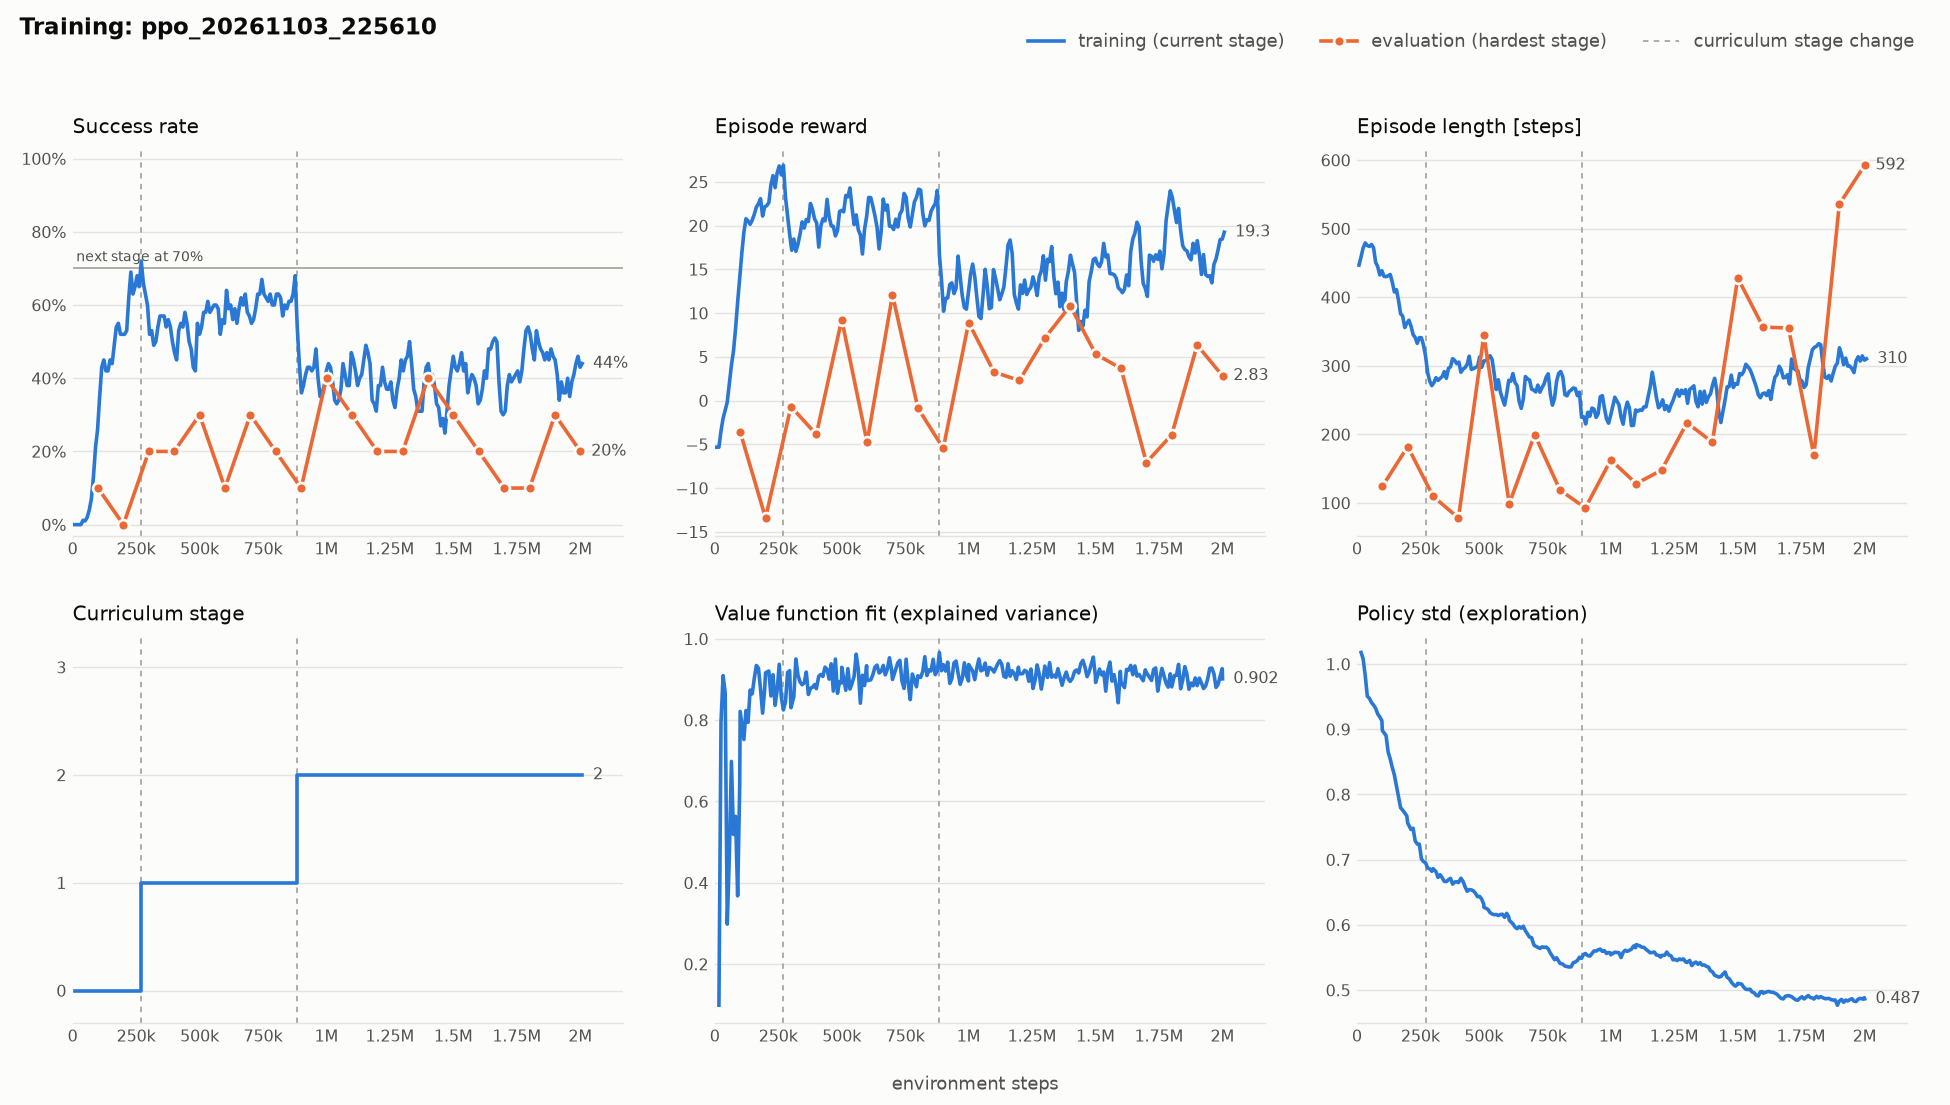
\includegraphics[width=\textwidth]{figures/training_ppo_20261103_225610.png}
\caption{2M-step run. Blue: training on the current stage; orange: evaluation
on the hardest stage (10 episodes each); dashed lines: stage changes.}
\label{fig:run}
\end{figure}

\begin{itemize}[leftmargin=*]
  \item \textbf{Curriculum:} stage $0\to1$ at about 270k steps and $1\to2$ at
        about 885k steps. On stage 2 the success rate stayed at about 35--55\%,
        so the last stage (rooms and maze) was never reached.
  \item \textbf{Evaluation:} of all 200 evaluation episodes, 21\% reached the
        goal, 73\% ended in a collision and 6\% in a timeout.
  \item \textbf{Learning:} the value function fits well (explained variance
        $\approx 0.9$) and the policy becomes more deterministic (std
        $1.0 \to 0.49$).
\end{itemize}

% ======================================================================
\section{Open issues and next steps}
% ======================================================================
\begin{enumerate}[leftmargin=*]
  \item \textbf{Collisions.} The 0.2\,m threshold leaves only 5--7\,cm around
        the robot body. Next: a small penalty for getting close to obstacles.
  \item \textbf{Plateau on stage 2.} Next: longer training or an intermediate
        stage between 3--8 and 8--15 obstacles.
  \item \textbf{Noisy evaluation.} 10 episodes per evaluation, and the best
        model is chosen by mean reward. Next: 50+ episodes on a fixed map set
        and selection by success rate.
  \item \textbf{No memory.} The policy sees only the current scan, which is
        likely to limit it in mazes. Next: frame stacking or a recurrent
        policy, then ROS~2 integration of the trained policy.
\end{enumerate}

% ######################################################################
\clearpage
\part*{Part II: reward, memory and curriculum (\code{PPO\_evoution\_and\_tweaks})}
\addcontentsline{toc}{part}{Part II}
% ######################################################################

% ======================================================================
\section{Summary}
% ======================================================================
The branch \code{PPO\_evoution\_and\_tweaks} (10--12 Nov, commits
\code{7dfa4c1}--\code{7cad22a}) addresses the collisions and the plateau
from Part~I. Every change was tested on its own (one change per run) and
compared on a fixed set of maps. The main outcomes:
\begin{itemize}[leftmargin=*]
  \item Collisions are now detected by physical contact, and a proximity
        penalty keeps the robot away from walls. Collisions in rooms dropped
        from 59\% to about 30\%.
  \item Diagnosis: the robot almost always succeeds when the goal is visible,
        and fails mostly when the goal is \emph{behind a wall}. Reward
        changes based on straight-line distance did not fix this.
  \item The decisive change was a \textbf{path-distance progress reward}
        (distance along free cells, used only in the reward). Rooms success
        rose from 21\% (Part~I model) to 42\%, and random maps from 70\% to
        77\%.
  \item A standard benchmark (\code{tb3-bench}) now evaluates every model on
        the same 600 maps in about 2 minutes.
  \item An overnight run with a wider maze (1\,m corridors) is in progress.
\end{itemize}

% ======================================================================
\section{Changes}
% ======================================================================

\paragraph{1. Contact-based collisions and proximity penalty (\code{7dfa4c1}).}
A collision is now a MuJoCo contact between any robot geom and a wall or
block, checked in every physics step, instead of a LiDAR reading
$\le 0.2$\,m. A linear proximity penalty (0 at 0.25\,m, $-0.1$ per step at
0.15\,m or closer) teaches the robot to keep a margin. The physics step was
changed to $10\times 0.005$\,s (still 0.05\,s per action), goal and collision
rewards to $+30$ and $-50$. A new \code{EpisodeStatsCallback} logs the
collision rate, timeout rate and closest obstacle distance to TensorBoard.
\emph{Tests:} touching a block ends the episode as a collision, the start pose
is not a collision, being close without contact is penalised but not a
collision. \emph{Effect:} the robot stopped driving into walls; it sometimes
waited in front of narrow gaps instead (timeouts).

\paragraph{2. Record-based progress and a rooms stage (\code{0834fdf}).}
Progress is rewarded only when the robot beats its best distance so far,
$10\cdot\max(0,\ d_\text{best}-d)$, so moving away and back is not rewarded
twice. A curriculum stage with rooms was added before the maze stage, and the
evaluation runs on that stage. 8 parallel environments. \emph{Effect:} faster
curriculum, but no better final result. A fixed-map diagnosis showed that the
robot reaches the goal in $\approx$98\% of episodes when the straight line to
the goal is free, but only in $\approx$60\% when it is blocked; all collisions
and timeouts happened in the blocked case.

\paragraph{3. Reward experiments that did not help (\code{4d3da88}, \code{c5f05c4}).}
Without the proximity penalty the timeout rate on stage~2 rose from 33\% to
50\%, so the penalty was kept. A larger time penalty ($-0.03$ instead of
$-0.01$) lowered random-map success at 2M steps from 75\% to 59\%, so it was
reverted.

\paragraph{4. Memory features in the observation (\code{6a3e741}, \code{534ad1e}).}
Two numbers derived from the robot's own history were added (observation
$41\to43$): \code{gap\_from\_best}, how much farther from the goal the robot
is than its best distance, and \code{stall}, the time since the last new best
distance (normalised to 10\,s). Neither uses map information. \emph{Effect:}
small and within seed noise; the best checkpoint reached 31\% in rooms
(Tab.~\ref{tab:experiments}).

\paragraph{5. Standard benchmark (\code{4f88e04}).}
\code{tb3-bench <model>} drives the model deterministically on 200 fixed maps
of each type (random, rooms, maze; map seeds 20000+) in 8 processes, about
2 minutes per model. It saves per-episode data, a summary, an outcome plot,
example trajectories and a comparison of all tested models in
\code{tests/benchmark/}. It also reports success separately for maps where
the goal is visible from the start and where it is hidden behind walls.

\paragraph{6. Fixed curriculum schedule (\code{8c327cc}).}
The threshold rule (70\% success over 100 episodes) depended on luck: the
training success on stage~2 is typically 40--55\%, so the threshold was only
crossed by a lucky streak. Two seeds with the same settings entered the maze
stage at 4.6M and 11.0M steps. Stages now change at fixed steps
(Tab.~\ref{tab:curriculum2}), so all runs are comparable. The maze stage was
removed for now. \emph{Effect:} on its own no improvement (rooms 22\% at 8M),
but rooms timeouts rose to 51\%: the robot did not find the doors.

\paragraph{7. Path-distance progress reward (\code{7cad22a}).}
The straight-line distance misleads the robot when the goal is in another
room: to get there it must first move away from the goal, towards a door.
The progress reward now uses the distance \emph{along free cells}: a
breadth-first search from the goal cell over the grid gives the number of
cells to the goal, times 0.5\,m (inside the goal cell the straight-line
distance is used). The map is used \textbf{only in the reward, during
training in simulation}; the policy still gets the same 43 inputs and no map.
This is the usual setup in embodied navigation benchmarks (e.g.\ the
geodesic-distance reward in Habitat PointNav). The memory features still use
the straight-line distance, so they carry no map information.

\paragraph{8. Wider maze.}
In the original maze the corridors are one cell (0.5\,m) wide, about 10\,cm
on each side of the robot; the models collided in 69--83\% of maze episodes.
\code{wide\_maze()} generates a $5\times5$ maze and scales it up twice, giving
1\,m corridors and walls. The benchmark maze maps now use this generator.

\begin{table}[H]
\centering\small
\begin{tabularx}{\textwidth}{@{}l X@{}}
\toprule
Observation (43) & 36 LiDAR readings, $v$, $\omega$, distance to goal, $\sin$/$\cos$ of the angle to goal, \code{gap\_from\_best}, \code{stall} \\
Reward per step & $10\cdot\max(0,\ p_\text{best}-p)$ with $p$ the path distance to the goal [m]; $-0.01$; proximity penalty $0\ldots-0.1$ below 0.25\,m \\
Episode end & goal $\le 0.2$\,m: $+30$; contact with a wall or block: $-50$; step limit (no penalty, truncation) \\
\bottomrule
\end{tabularx}
\caption{\code{NavEnv} at the end of Part II (changes from Part~I).}
\end{table}

\begin{table}[H]
\centering\small
\begin{tabular}{@{}c l c c c c@{}}
\toprule
Stage & Map types & Obstacles & Min.\ distance & Step limit & Starts at \\
\midrule
0 & random & 0--3 & 2 cells & 500 & 0 \\
1 & random & 3--8 & 3 cells & 500 & 0.5M \\
2 & random & 8--15 & 5 cells & 500 & 1M \\
3 & random, rooms & 8--15 & 5 cells & 1000 & 2.5M \\
4 & random, rooms, wide maze & 8--15 & 5 cells & 1500 & 16M (overnight run) \\
\bottomrule
\end{tabular}
\caption{Curriculum with a fixed schedule.}
\label{tab:curriculum2}
\end{table}

% ======================================================================
\section{Results}
% ======================================================================

\paragraph{Intermediate experiments.} Before the benchmark existed, models
were compared on 100 fixed maps per type (the first 100 maps of the
benchmark, original narrow maze).

\begin{table}[H]
\centering\small
\begin{tabular}{@{}l l c c@{}}
\toprule
Run & Change & Random maps [\%] & Rooms [\%] \\
\midrule
\code{ppo\_20261110\_220127} & record progress, rooms stage & 71 / 63 (3M / 5M) & 20 / 16 \\
\code{ppo\_20261111\_202451} & + \code{gap\_from\_best} & 70 / 63 (3M / 5M) & 25 / 22 \\
\code{stall\_seed0} & + \code{stall} & 70 / 73 / 68 (3M / 5M / 12M) & 31 / 27 / 21 \\
\code{stall\_seed1} & + \code{stall}, other seed & 75 / 73 / 72 (3M / 5M / 12M) & 24 / 22 / 20 \\
\bottomrule
\end{tabular}
\caption{Goal reached on fixed maps (deterministic policy).}
\label{tab:experiments}
\end{table}

\paragraph{Benchmark.} Table~\ref{tab:bench} and Fig.~\ref{fig:bench} compare
the final Part~I model with the main models of Part~II on the same 600 maps.
The maze column uses the new wide maze, on which none of these models was
trained.

\begin{table}[H]
\centering\small
\begin{tabular}{@{}l c c c c c@{}}
\toprule
& \multicolumn{2}{c}{Random maps} & \multicolumn{3}{c}{Rooms} \\
\cmidrule(lr){2-3}\cmidrule(lr){4-6}
Model & goal & goal hidden & goal & goal hidden & collision / timeout \\
\midrule
Part I final (\code{ppo\_20261103\_225610}, 2M) & 70 & 62 & 21 & 14 & 59 / 20 \\
memory features (\code{stall\_seed0}, 3M) & 73 & 65 & 30 & 23 & 30 / 40 \\
fixed schedule (\code{fixed\_s0}, 8M) & 69 & 59 & 22 & 14 & 26 / 51 \\
\textbf{path reward} (\code{pathreward\_s0}, 16M) & \textbf{77} & \textbf{71} & \textbf{42} & \textbf{37} & 35 / 24 \\
\bottomrule
\end{tabular}
\caption{Benchmark, 200 maps per type, in \%. ``Goal hidden'': the goal is
not visible from the start (blocked straight line).}
\label{tab:bench}
\end{table}

\begin{figure}[H]
\centering
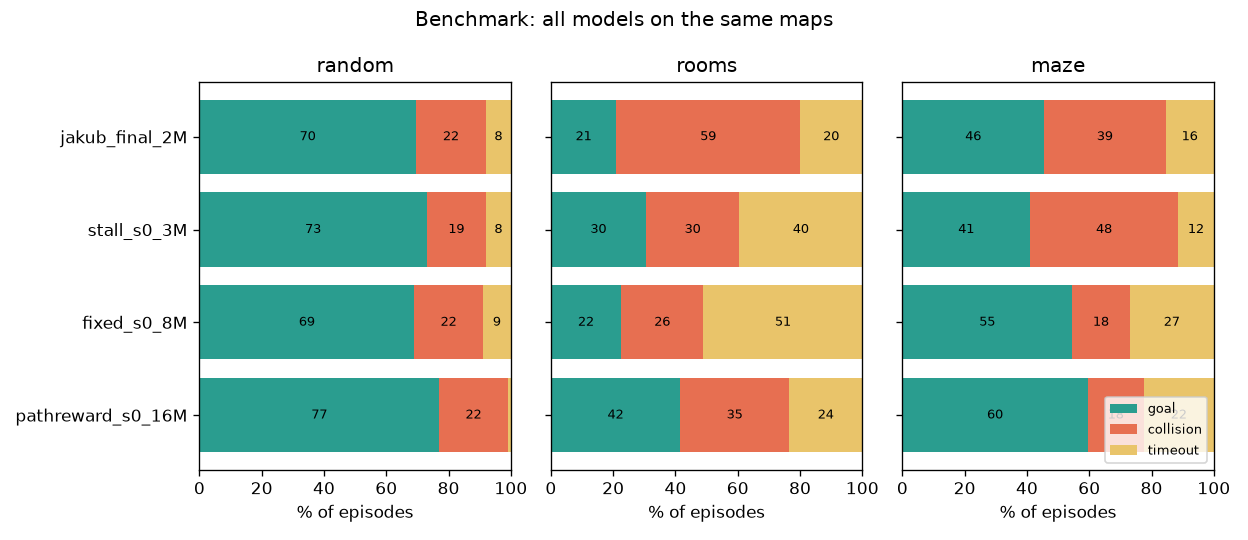
\includegraphics[width=\textwidth]{figures/benchmark_comparison.png}
\caption{Benchmark outcomes of all models (green: goal, red: collision,
yellow: timeout).}
\label{fig:bench}
\end{figure}

\begin{figure}[H]
\centering
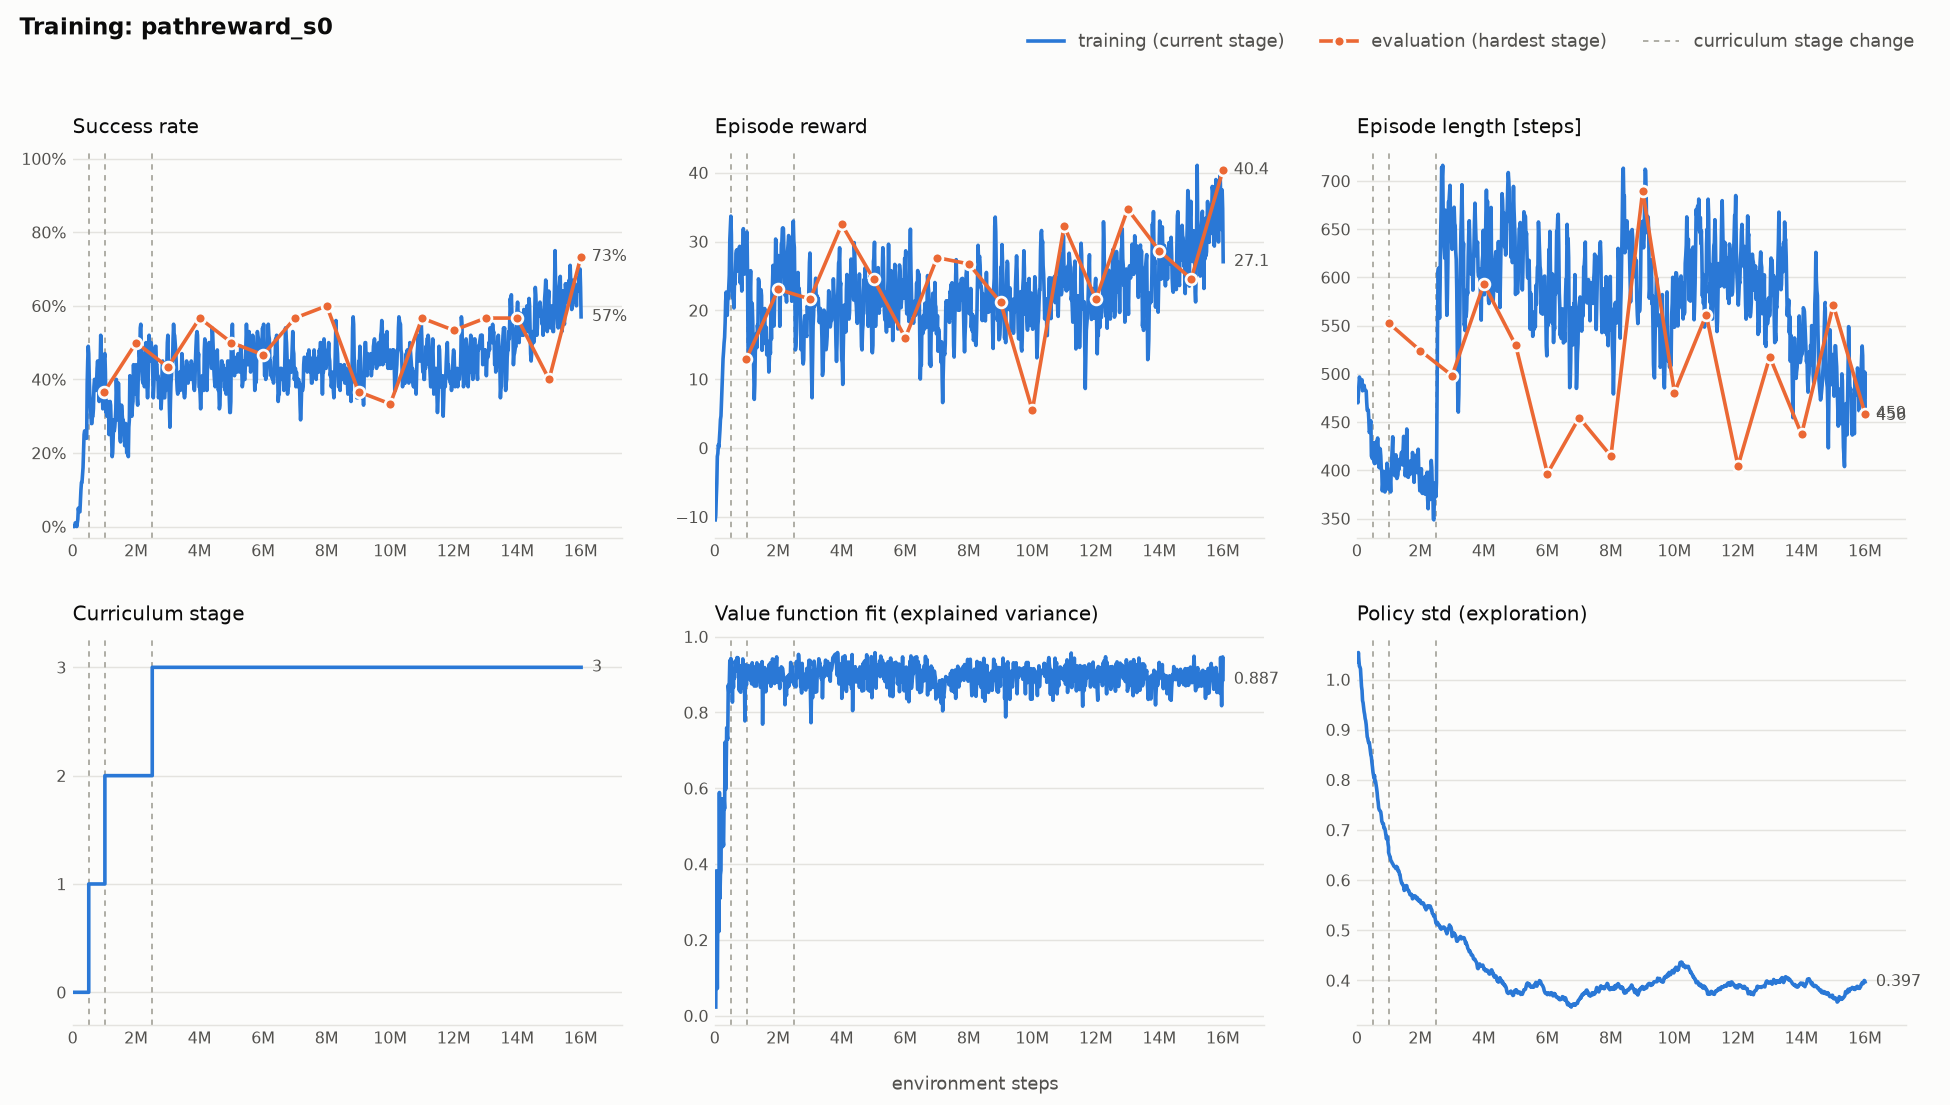
\includegraphics[width=\textwidth]{figures/training_pathreward_s0.png}
\caption{Run \code{pathreward\_s0} (16M steps). The training success rate
stays at 40--50\% until about 14M steps and then rises to about 60\%;
the run ended while it was still improving.}
\label{fig:pathreward}
\end{figure}

\begin{figure}[H]
\centering
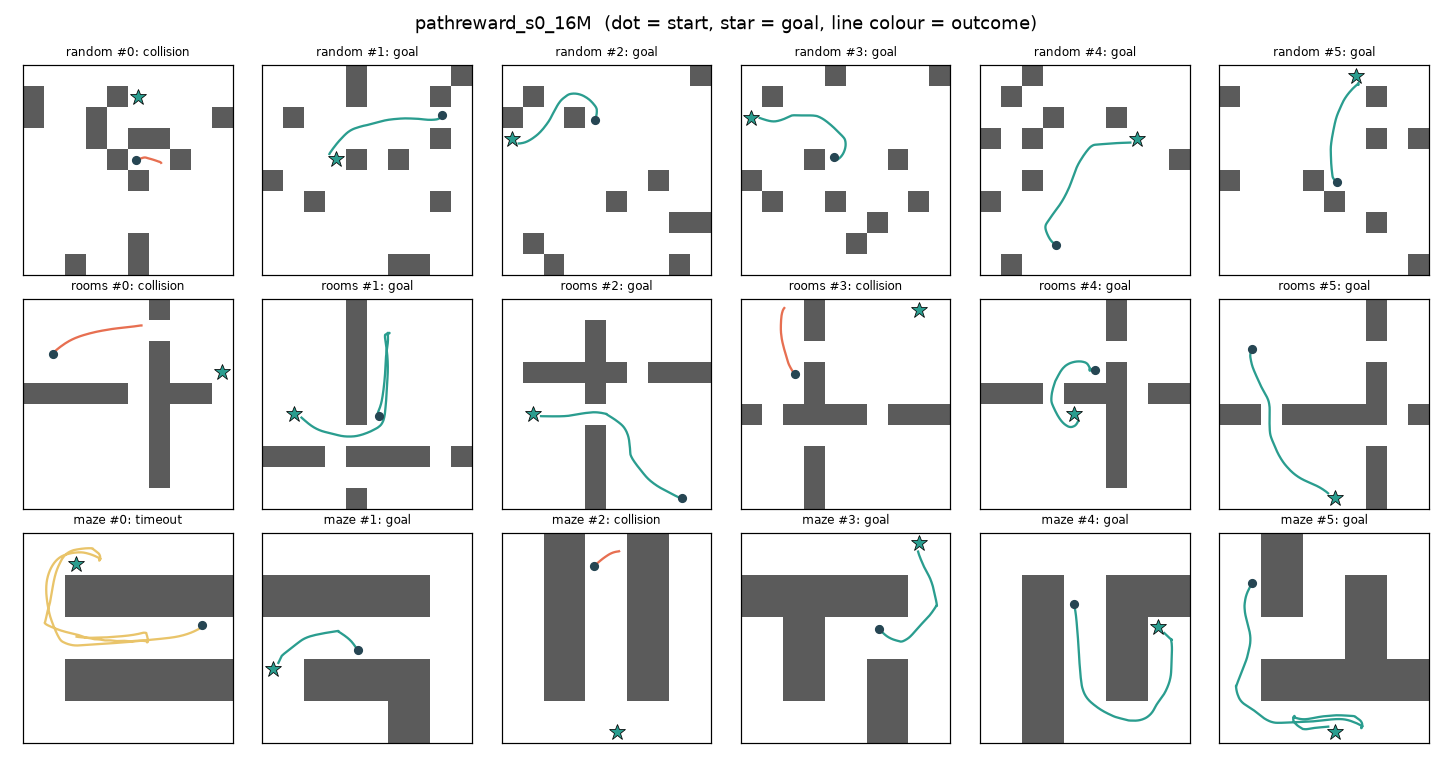
\includegraphics[width=\textwidth]{figures/trajectories_pathreward_s0_16M.png}
\caption{Example paths of \code{pathreward\_s0} on the first six benchmark
maps of each type.}
\end{figure}

\paragraph{Observations.}
\begin{itemize}[leftmargin=*]
  \item \textbf{Seed noise} between two runs with the same settings is
        5--9 percentage points, so a change needs two seeds or a large
        effect. The path reward (+11--21 points in rooms) is the first change
        clearly above this level.
  \item \textbf{Training success is lower than test success} (about 50\% vs
        about 75\% on random maps), because training samples random actions
        and the test uses the mean action.
  \item \textbf{\code{best\_model.zip} is unreliable}: it is chosen by the
        mean reward of 30 episodes. On 100 fixed random maps the Part~I best
        model reaches 54\%, its final model 74\%. Models are now compared with the
        benchmark only.
  \item With the straight-line reward, longer training did not help in rooms
        (results fell from about 30\% at 3M to about 20\% at 12M).
\end{itemize}

% ======================================================================
\section{Run in progress and next steps}
% ======================================================================
\paragraph{Overnight run \code{pathreward\_maze\_s0}.} Same settings as
\code{pathreward\_s0} (path reward, fixed schedule, seed 0) for the first
16M steps, then the wide maze is added (stage~4), 30M steps in total. The
16M checkpoint gives a second measurement of the current setup; the rest
shows the effect of the maze stage and of longer training. Without any maze
training, \code{pathreward\_s0} already reaches the goal in 60\% of the wide
maze maps (18\% collisions).

\begin{enumerate}[leftmargin=*]
  \item Benchmark the overnight checkpoints (16M, 20M, 25M, 30M).
  \item Repeat the best setup with a second seed.
  \item Rooms remain the bottleneck (35\% collisions, 24\% timeouts). Next
        candidates, one at a time: a recurrent policy (LSTM) for longer
        memory, more LiDAR rays or range.
  \item Export the trained policy to ROS~2.
\end{enumerate}

\end{document}
